\documentclass[thesis.tex]{subfiles}

\begin{document}

\chapter{Prerequisites}\label{chap:preq}

This chapter lists and describes the necessary topics to follow this thesis. It explains SCION's structure, functionality and details about the component as for example the border router. SCIONLab itself and its work is also outlined. At last, a short description about Prometheus and its used features will be given.

\section{SCION} \cite{SCIONPaper} \cite{SCIONBook}

SCION, an acronym for \textbf{S}calability, \textbf{C}ontrol and \textbf{I}solation \textbf{O}n \textbf{N}ext-generation networks, provides a green-field solution for problems of the current Internet, which is named in this content as the \textit{legacy internet}. The main difference between them is \textit{path-transparency}. In the current existing IP routing protocol the end-hosts cannot chose a path, but must rely on the router between them to find a good path. This leads to the problem, that the receiver cannot verify, if the packets were modified nor if the taken path was trustworthy. SCION allows the end hosts to chose between communication paths and also to see the path of a packet on the end-host. The fundamental change needs a different organization of the network nodes, which will be described in this part.

\autoref{fig:prequirement:scionStructure} shows an example SCION network from \cite{SCIONPaper}. This topology consists of \textbf{Is}olation \textbf{D}omains (ISD) and each node of it is considered an \textbf{A}utonomous \textbf{S}ystem (AS). They represent exactly one physical end-host, a whole companies network or an \textbf{I}nternet \textbf{S}ervice \textbf{P}rovider (ISP)'s network. Each ISD is administered and initially created by a small group of ASes, which are referred to \textit{Core} ASes and forms the \textit{Core} of an ISD. They are responsible to define a policy which applies to all member of the ISD and is called the \textbf{T}rust \textbf{R}oot \textbf{C}onfiguration (TRC). Concluding this each ISD has its own rules to create connection and also defines the name the ISD. The Core ASes are also connect with other ISDs and link their ISDs to them. Additionally an AS can belong to multiple ISDs at one time, which is the case for the AS \textbf{H}.

An AS needs to know the path to another AS to communicate to them. This routing problem is solved with a process called \textit{beaconing}. A core AS announces such a beaconing inside its ISDs and learns the different paths from a core AS to a non-core AS. The ASes respond to this beaconing and over time the topology is created. On the other side, a non-core AS explores by beaconing the paths to the core-AS. The same procedure is done for inter-ISD communication by the core-ASes. The up-segment from a non-core AS to the Core and the down-segment from the beaconing of a core-AS are merged together and send to the \textit{path-server}. This component handles routing requests from one AS to another AS and responds with a set of possible paths to take. The elements of this set depend on the TRC of the ISD. For example, one ISD does not want to enable multiple path communication and only responds with the first available path.

One advantage of this structured routing is that a communication does not leave an ISD when it is not necessary. This enables to create ISDs for different security or efficiency scenarios. Packets are only routed in a trusted zone when they need to be. The legacy internet do not guarantee this behavior. A packet from OvGU-Magdeburg to ETH-Zuerich could be routed over different location in the world without control over it. If both of them were inside one ISD containing only research institutes, than the packet would be guaranteed to not leave this ISD because it is not necessary.

Another advantage is the possibility to choose an alternative way. This is interesting in cases a path segment has a failure and should be avoided for different reasons like malicious attacks or technical failures. The legacy internet relies on the Border-Gateway-Protocol \todo{Quelle dafür einfügen}, when was inspected by many researcher for its fault-tolerance and stability. \todo{Dort die quellen einfügen aus SCIONBook}. It was also shown in \cite{Sahoo.2006} that the reaction time (convergence) for realistic topologies takes seconds to minutes for the protocol to adjust to failures. A similar result was given by \cite{Labovitz.2001} of a delay of 3 minutes for 30\% the cases and even higher as 15 minutes in total. In SCION this slow reaction problem is minimized by letting the user choose different path. If one path is not responding the node can request another path and use that. 

\begin{figure}
	\centering
	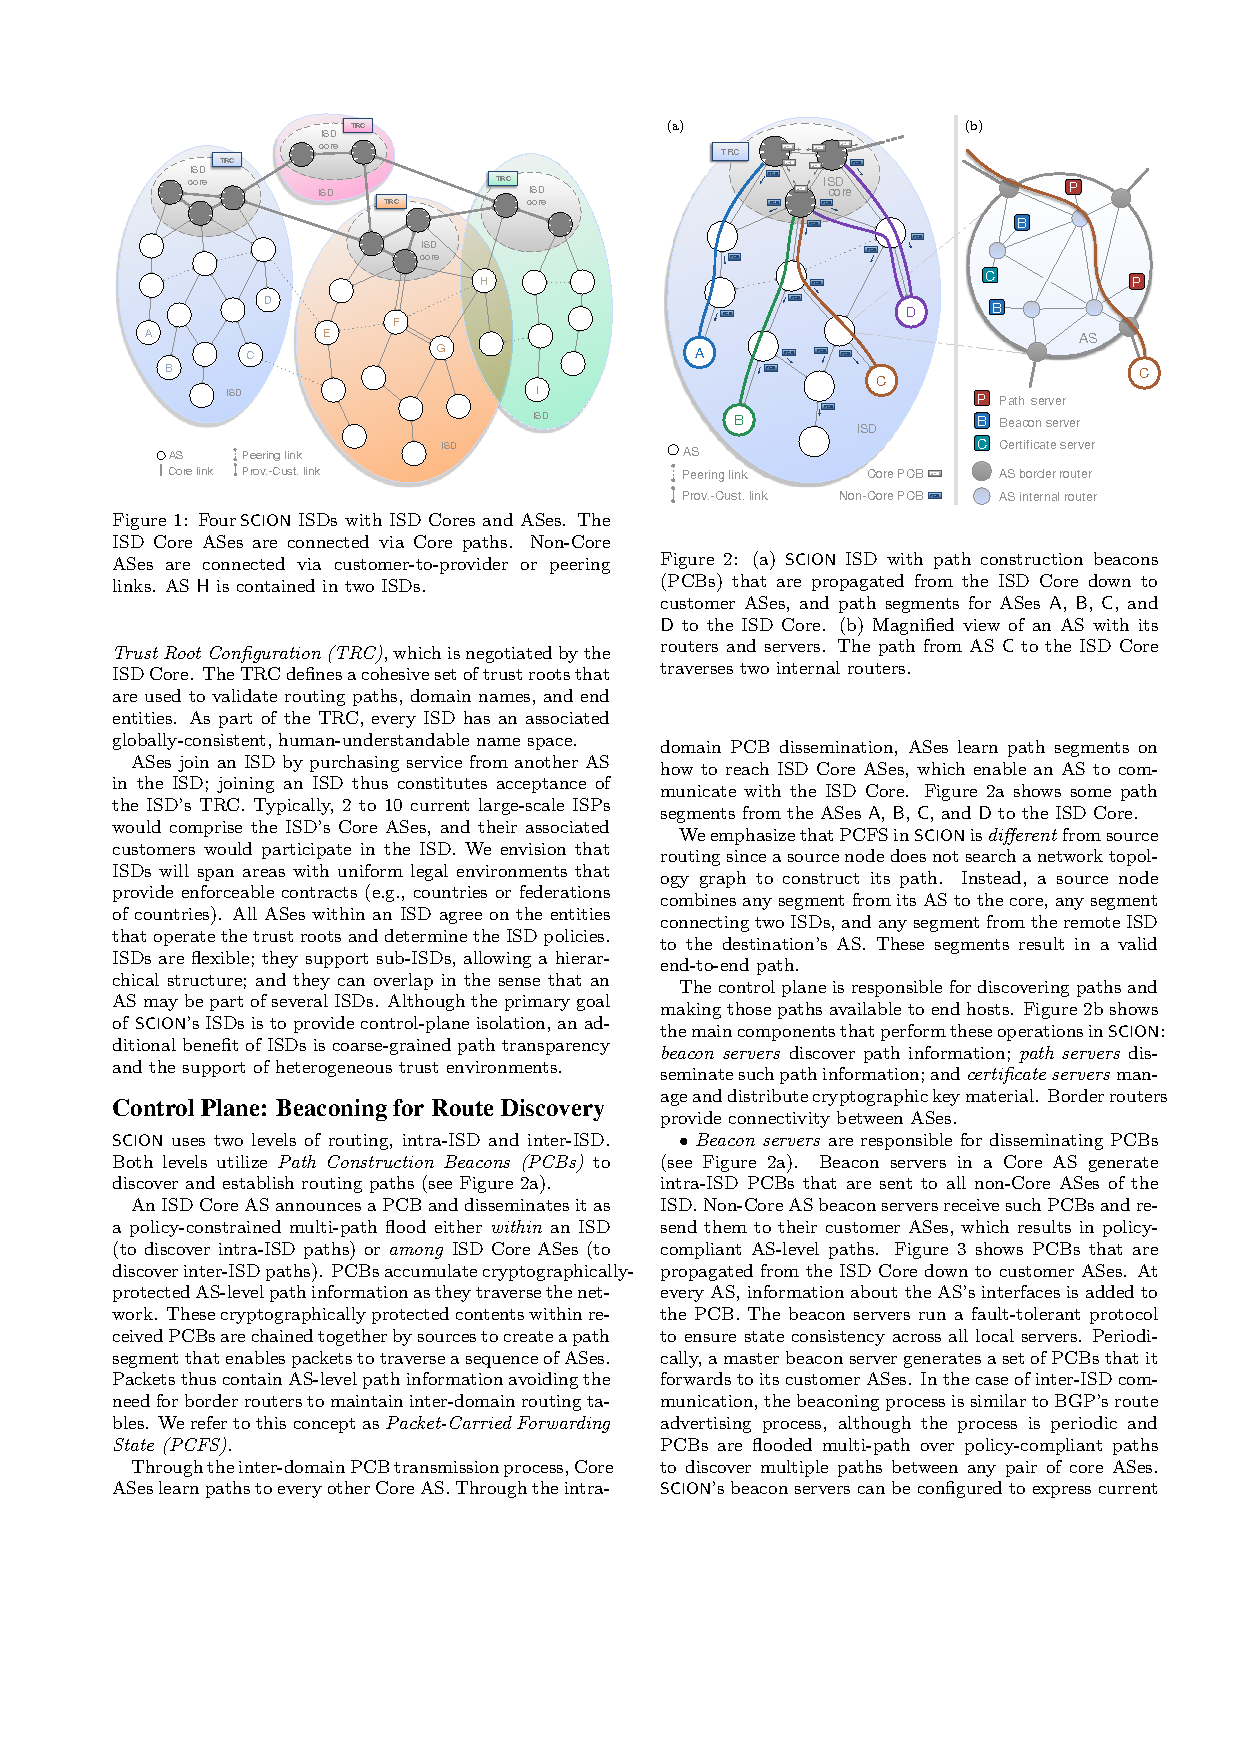
\includegraphics[trim=19mm 214mm 105mm 19mm ,clip,width=0.5\linewidth]{2015-SCION-short_3.pdf}
	\caption{Four SCION ISDs with ISD Cores and ASes \cite{SCIONPaper}}
	\label{fig:prequirement:scionStructure}
\end{figure}

shortcomings [25, 117, 216,
219] and especially lacks integrity protection for routing update messages.
Maliciously acting
\begin{easylist}
    \MyListProperties
    # SCION
    ## Origins of SCION
    ## Structure of SCION
    ## \textit{Figure example topology}
    ## Explain relevant components of an AS
    ### Path Server + Path Discovery
    ### Border Router
    ## SCIONLab
    ### Goal \& How it works
    ### Coordinator in ETH Zurich
    ## Multipath method
    ### How does it work
    ### \textit{Figure of example}
    ### Explanation of example
    ### Difference to legacy methods
    # Other prerequisites
\end{easylist}

\subfilebib % Makes bibliography available when compiling as subfile
\end{document}